%%%%%%%%%%%%%%%%%%%%%%%%%%%%%%%%%%%%%%%%%
% Wenneker Assignment
% LaTeX Template
% Version 2.0 (12/1/2019)
%
% This template originates from:
% http://www.LaTeXTemplates.com
%
% Authors:
% Vel (vel@LaTeXTemplates.com)
% Frits Wenneker
%
% License:
% CC BY-NC-SA 3.0 (http://creativecommons.org/licenses/by-nc-sa/3.0/)
% 
%%%%%%%%%%%%%%%%%%%%%%%%%%%%%%%%%%%%%%%%%

%----------------------------------------------------------------------------------------
%	PACKAGES AND OTHER DOCUMENT CONFIGURATIONS
%----------------------------------------------------------------------------------------

\documentclass[11pt]{scrartcl} % Font size
\usepackage{algorithmic}
%%%%%%%%%%%%%%%%%%%%%%%%%%%%%%%%%%%%%%%%%
% Wenneker Assignment
% Structure Specification File
% Version 2.0 (12/1/2019)
%
% This template originates from:
% http://www.LaTeXTemplates.com
%
% Authors:
% Vel (vel@LaTeXTemplates.com)
% Frits Wenneker
%
% License:
% CC BY-NC-SA 3.0 (http://creativecommons.org/licenses/by-nc-sa/3.0/)
% 
%%%%%%%%%%%%%%%%%%%%%%%%%%%%%%%%%%%%%%%%%

%----------------------------------------------------------------------------------------
%	PACKAGES AND OTHER DOCUMENT CONFIGURATIONS
%----------------------------------------------------------------------------------------

\usepackage{amsmath, amsfonts, amsthm} % Math packages

\usepackage{listings} % Code listings, with syntax highlighting

\usepackage[english]{babel} % English language hyphenation

\usepackage{graphicx} % Required for inserting images
\graphicspath{{Figures/}{./}} % Specifies where to look for included images (trailing slash required)

\usepackage{booktabs} % Required for better horizontal rules in tables

\numberwithin{equation}{section} % Number equations within sections (i.e. 1.1, 1.2, 2.1, 2.2 instead of 1, 2, 3, 4)
\numberwithin{figure}{section} % Number figures within sections (i.e. 1.1, 1.2, 2.1, 2.2 instead of 1, 2, 3, 4)
\numberwithin{table}{section} % Number tables within sections (i.e. 1.1, 1.2, 2.1, 2.2 instead of 1, 2, 3, 4)

\setlength\parindent{0pt} % Removes all indentation from paragraphs

\usepackage{enumitem} % Required for list customisation
\setlist{noitemsep} % No spacing between list items

%----------------------------------------------------------------------------------------
%	DOCUMENT MARGINS
%----------------------------------------------------------------------------------------

\usepackage{geometry} % Required for adjusting page dimensions and margins

\geometry{
	paper=a4paper, % Paper size, change to letterpaper for US letter size
	top=2.5cm, % Top margin
	bottom=3cm, % Bottom margin
	left=3cm, % Left margin
	right=3cm, % Right margin
	headheight=0.75cm, % Header height
	footskip=1.5cm, % Space from the bottom margin to the baseline of the footer
	headsep=0.75cm, % Space from the top margin to the baseline of the header
	%showframe, % Uncomment to show how the type block is set on the page
}

%----------------------------------------------------------------------------------------
%	FONTS
%----------------------------------------------------------------------------------------

\usepackage[utf8]{inputenc} % Required for inputting international characters
\usepackage[T1]{fontenc} % Use 8-bit encoding

\usepackage{fourier} % Use the Adobe Utopia font for the document

%----------------------------------------------------------------------------------------
%	SECTION TITLES
%----------------------------------------------------------------------------------------

\usepackage{sectsty} % Allows customising section commands

\sectionfont{\vspace{6pt}\centering\normalfont\scshape} % \section{} styling
\subsectionfont{\normalfont\bfseries} % \subsection{} styling
\subsubsectionfont{\normalfont\itshape} % \subsubsection{} styling
\paragraphfont{\normalfont\scshape} % \paragraph{} styling

%----------------------------------------------------------------------------------------
%	HEADERS AND FOOTERS
%----------------------------------------------------------------------------------------

\usepackage{scrlayer-scrpage} % Required for customising headers and footers

\ohead*{} % Right header
\ihead*{} % Left header
\chead*{} % Centre header

\ofoot*{} % Right footer
\ifoot*{} % Left footer
\cfoot*{\pagemark} % Centre footer
 % Include the file specifying the document structure and custom commands
%\usepackage[demo]{graphicx}
%\usepackage{caption}
\usepackage{subcaption}
\usepackage{float}
\usepackage{listings}
\usepackage[showframe=true]{geometry}
\usepackage{changepage}

%----------------------------------------------------------------------------------------
%	TITLE SECTION
%----------------------------------------------------------------------------------------

\title{	
	\normalfont\normalsize
	\textsc{Università degli Studi di Trieste}\\ % Your university, school and/or department name(s)
	\vspace{25pt} % Whitespace
	\rule{\linewidth}{0.5pt}\\ % Thin top horizontal rule
	\vspace{20pt} % Whitespace
	{\huge First FHPC Assignment}\\ % The assignment title
	\vspace{12pt} % Whitespace
	\rule{\linewidth}{2pt}\\ % Thick bottom horizontal rule
	\vspace{12pt} % Whitespace
}

\author{\LARGE Nicola Domenis} % Your name

\date{\normalsize\today} % Today's date (\today) or a custom date

\begin{document}

\maketitle % Print the title

%----------------------------------------------------------------------------------------
%	FIGURE EXAMPLE
%----------------------------------------------------------------------------------------

\section{Preview}
 
In this assignment we will present the following subjects:

\begin{itemize}
	\item the analysis of the computational power of our laptop and smartphone;
	\item the analysis of a strong scaling model for a simple addition problem;
	\item the resolution of a scalability problem for a simple parallel code that computes pi;
	\item the parallel implementation of the above addition model;
	\item the scalability of the above addition program.
\end{itemize}


%------------------------------------------------
\section{section 0}
\subsection{Laptop theoretical peak performance}

We want to calculate the theoretical peak performance of our own portable computer by using the formula \textbf{theoretical peak performance = clock frequency x FLOPs x number of cores}.
We gather that \textbf{clock frequency} $= 2.90 Ghz$, \textbf{FLOPs} = 16 and \textit{number of cores} $= 2$ for our computer architecture, an intel i7 with a Kaby Lake micro-architecture; thus we compute \textbf{theoretical peak performance} $= 92.8 GFlops/s$

\begin{table}[H]
		\begin{tabular}[H]{l| l| l| l| l| l }
			&Your model&CPU&Frequency&Number of Cores&Peak Performance\\
			laptop& Asus F556U & Intel Core i7-7500 &$2.90$ GHz&2&92.8 GFLOPs/s
		\end{tabular}
	\label{Result}
\end{table}
%\end{adjustwidth}
%\end{figure}

\subsection{Smartphone theoretical peak performance}
We installed "`Mobile Linpack"' app and we run a few tests. We report here some results,even on repeated trials: 
%\begin{figure}
\begin{adjustwidth}{-2cm}{}
	\begin{tabular}[H]{l| p{0.2\textwidth}| l |l| p{0.2\textwidth}|l }
		\hline
			&Model& Sustained performance&Matrix size&Peak performance&Memory\\
			\hline
			Cellphone&Samsung Galaxy XCover 4 &114,81 Mflops/s &250 &not calculated(we didn't find the FLOPs of the cpu, which is a quad-core processor with a 1.4 Ghz clock frequency)&16,00 GB\\
			& &145.53 Mflop/s&500& &\\
			& &157.5 Mflop/s&800& &\\
			& &201.32 Mflop/s&800& &\\
			& &155.93 Mflop/s&900& &\\
			& &109.88 Mflop/s&1000& &\\
			& &103.14 Mflop/s&2000& &\\
		\end{tabular}
\end{adjustwidth}
%\end{figure}

\subsection{Laptops,smartphones and the top 500}
Let's check now whether our devices would have competed with the Top500 supercomputers in the past:
%\begin{figure}
\begin{adjustwidth}{-2cm}{}
	\begin{tabular}[H]{p{0.15\textwidth}| p{0.15\textwidth}| p{0.15\textwidth} | p{0.3\textwidth}| p{0.3\textwidth}}
		\hline
			&Model&Performance&Top 500 year\& position&number 1 HPC system\\
			\hline
			Smartphone&Samsung Galaxy XCover 4 &201,32 Mflops/s &does not enter in the top500 on the first year of measurement, the 500th Supercomputer has an Rmax of 0.5 GFlops/s (equal to 2.4 times our smartphone peak performance)& Numerical Wind Tunnel,Fujitsu National Aerospace Laboratory of Japan is first in the year 1993 with a Rmax equal to 124.0 GFlops/s (equal to 616 times our cellphone's sustained peak performance)\\
			\hline
			Laptop&ASUS F556U&92.8 GFLOPs/s& 3rd position at nov 1993. Remains in the top 10 until nov 1996 & We have the same top 1  position with a Rpeak equal to 235.8 GFlops/s(equal to 2.5 times our laptop's theoretical peak performance)\\
		\end{tabular}
\end{adjustwidth}
%\end{figure}

%\begin{table}
	%\centering
		%\begin{tabular}{l| l| l |l| l| l}
			%&Model& Sustained performance&Matrix size&Peak performance&Memory\\
			%Cellphone&Samsung Galaxy XCover 4 &114,81 Mflops/s &250 &not calculated&16,00 GB
			%&&145.53 Mflop/s&500&&
			%&&157.5 Mflop/s&800&&
			%&&109.88 Mflop/s&1000&&
		%\end{tabular}
	%\label{Quick test parameters and results}
%\end{table}

%----------------------------------------------------------------------------------------
%	TEXT EXAMPLE
%----------------------------------------------------------------------------------------

\section{Section 1}

\subsection{Model for a serial and parallel summation of n numbers}
Here we discuss about modeling a simple program which consists of summing n numbers.
A simple pseudocode for the serial program would be:


\begin{algorithmic}

\STATE {Data:array $A[]$ of values}
\FOR{i from 1 to n} \STATE {sum = sum + A[i]} \ENDFOR
\RETURN{sum}
\end{algorithmic}

If we choose $T_{comp}$ as the time to compute a floating point operation we could calculate the total time of a serial computation as
$T_s = N * T_{comp}$,where the code simply computes N times(the size of the problem) the sum of two values.

For the parallel program we complicate a little the execution:

\begin{algorithmic}

\STATE {Data:array $A[]$ of values}
\STATE {Environment: p parallel processors}
\IF {Master process}

		\STATE{Read and Split $A[]$ into p subarrays $A_i[]$}
		\STATE{Send $p-1$ subarrays to the other $p-1$ processors}
		\FOR{i from $1$ to n/p} \STATE {$sum_0 = sum_0 + A_0[i]$} \ENDFOR
		\STATE{Collect the resulting $p-1$ values $sum_i$ from the processors}
		\FOR{i from $1$ to p} \STATE {$sum = sum + sum_i$} \ENDFOR
\ENDIF
\IF {Slave process}
	\STATE{Receive subarrays $A_i[]$ from the Master process}
	\FOR{i from 1 to n/p} \STATE {$sum_i = sum_i + A_i[i]$} \ENDFOR
	\STATE{Send $sum_i$ back to the Master process}
\ENDIF
\RETURN{sum}
\end{algorithmic}

If we define the times $T_{read}$ to indicate the time needed to read a variable,and $T_{comm}$ to indicate the time needed to communicate a variable, we can deduce the theoretical execution time of the model:
\  
\begin{algorithmic}
		\STATE{Read $A[]$}
		\STATE{EXECUTION TIME: $T_{read}$}
\end{algorithmic}
\ 
\begin{algorithmic}
		\STATE{Send $p-1$ subarrays to the other $p-1$ processors}
		\STATE{EXECUTION TIME: $T_{comm}*(p-1)$}
\end{algorithmic}
\ 

\begin{algorithmic}

\FOR{i from $1$ to $n/p$} \STATE {$sum_i = sum_i + A_i[i]$} \ENDFOR
\STATE{EXECUTION TIME: $n/p * T_{comp}$}
\STATE{This is a parallel execution, the subarrays are added inside each processor}	
\end{algorithmic}

\ 
\begin{algorithmic}
\STATE{Send $sum_i$ back to the Master process}
\STATE{EXECUTION TIME: $(p-1)*T_{comm}$}
\end{algorithmic}
\ 
\begin{algorithmic}
		\FOR{i from $1$ to p} \STATE {$sum = sum + sum_i$} \ENDFOR
		\STATE{EXECUTION TIME: $(p-1)*T_{comp}$}
\end{algorithmic}

The total sum of the execution times gives $T_p = T_{read} + (p-1+n/p)*T_{comp}+2*T_{comm}(p-1)$. We can calculate it with the theoretical values $T_{comp} =2 \times 10^{-9}$,$T_{read}= 1 \times 10^{-4}$ and $T_{comm}= 1 \times 10^{-6}$
%----------------------------------------------

\subsection{Scalability of the Model}

Once we have the theoretical $T_p$ and $T_s$ we can calculate the Speedup given by the formula $Speedup(p)=T_s/T_p$ . We give the following plots on the variable $p$:

%\begin{figure}
%\centering
%\begin{subfigure}{.5\textwidth}
	%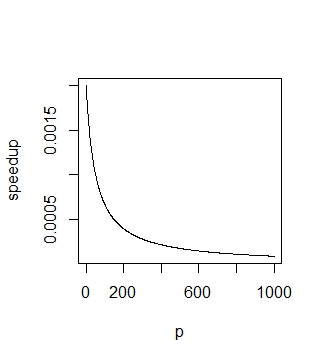
\includegraphics[width=0.5\columnwidth]{Rplot_speedup_4} % Example image
	%\caption{Speedup for $N=10^2$,maximum: $speedup = 0.00199$ at $p = 1$}
%\end{subfigure}%
%\begin{subfigure}{.5\textwidth}
 %% [h] forces the figure to be output where it is defined in the code (it suppresses floating)
	%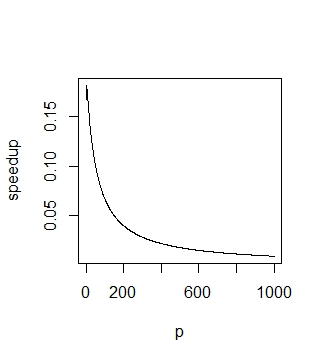
\includegraphics[width=0.5\columnwidth]{Rplot_speedup_3} % Example image
	%\caption{Speedup for $N=10^4$,maximum: $speedup = 0.180$ at $p = 3$}
 %\end{subfigure}
%\end{figure}

\begin{figure}[H] % [h] forces the figure to be output where it is defined in the code (it suppresses floating)
	\centering
	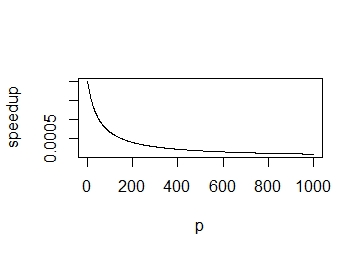
\includegraphics[width=0.6\columnwidth]{Rplot_speedup_sum_2} % Example image
	\caption{Speedup for $N=10^2$,maximum: $speedup = 0.002$ at $p = 1$}
\end{figure}


\begin{figure}[H] % [h] forces the figure to be output where it is defined in the code (it suppresses floating)
	\centering
	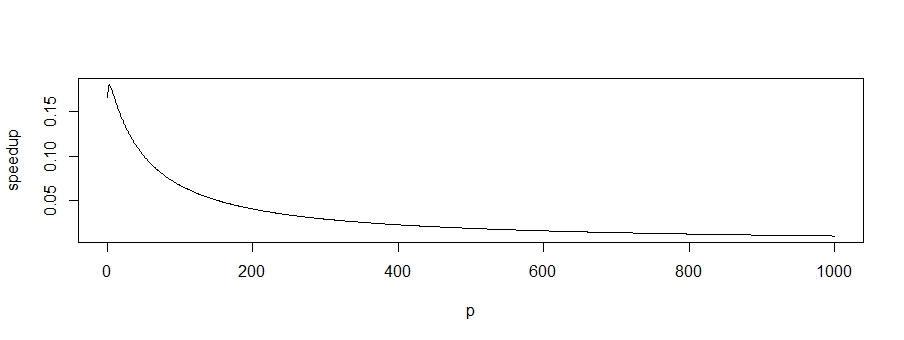
\includegraphics[width=0.6\columnwidth]{Rplot_speedup_sum_4} % Example image
	\caption{Speedup for $N=10^4$,maximum: $speedup = 0.181$ at $p = 3$}
\end{figure}
\begin{figure}[H] % [h] forces the figure to be output where it is defined in the code (it suppresses floating)
	\centering
	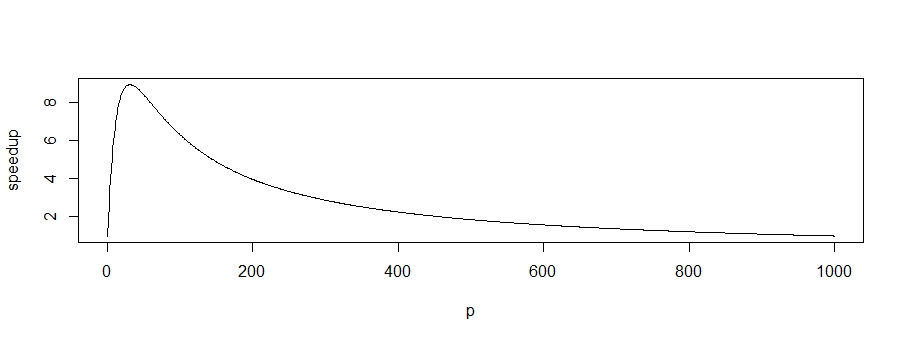
\includegraphics[width=0.6\columnwidth]{Rplot_speedup_sum_6} % Example image
	\caption{Speedup for $N=10^6$,maximum: $speedup = 8.91$ at $p = 32$}
\end{figure}
\begin{figure}[H] % [h] forces the figure to be output where it is defined in the code (it suppresses floating)
	\centering
	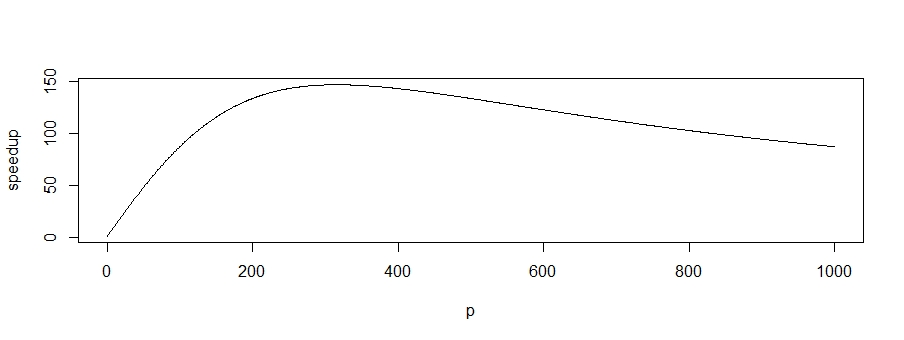
\includegraphics[width=0.6\columnwidth]{Rplot_speedup_sum_8} % Example image
	\caption{Speedup for $N=10^8$,maximum: $speedup = 147$ at $p = 316$}
\end{figure}
\begin{figure}[H] % [h] forces the figure to be output where it is defined in the code (it suppresses floating)
	\centering
	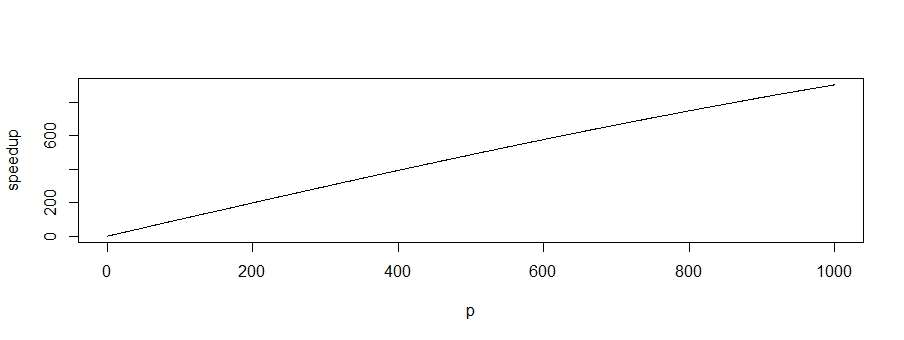
\includegraphics[width=0.6\columnwidth]{Rplot_speedup_sum_10} % Example image
	\caption{Speedup for $N=10^{10}$,maximum: $speedup = 905$ at $p = 1000$}
\end{figure}

We notice that as we increase N we get closer to a case of perfect scaling on our number of processors. As N grows, adding a certain number of processors accelerates the calculations almost linearly.
If N is low,instead, we see that the problem starts improving around $N=10^6$, where the speedup grows up to a maximum, and then decreases:the communication time surpasses the advantage of the parallelization, thus lowering the speedup.
 Simply adding processors to the calculus will not speed up the process because the time it takes to the master node to assign the subarrays to the slaves and then read to read back the results grows as well.
The algorithm performs well if :
\begin{itemize}
	\item p corresponds to the maximum speedup;
	\item the maximum speedup is greater than 1: it makes the parallelization convenient,otherwise $T_p>T_s$ and a parallel execution would take more time than the serial one.
\end{itemize}
%------------------------------------------------
\section{Section 2}

\subsection{\textit{mpi\_pi.c} and \textit{pi.c} execution}
We start by executing the two codes \textit{pi.c} and \textit{mpi\_pi.c}. We have:

\begin{lstlisting}[language=bash]
  
$ g++ pi.c -o pi.x
$ ./pi.x 10000000

 # of trials = 10000000 , estimate of pi is 3.141396400 

 # walltime : 0.19000000 
\end{lstlisting}
And the parallel file:
\begin{lstlisting}[language=bash]
$ mpicc mpi_pi.c -o mpi_pi.x
$ mpirun -np 10 ./mpi_p.x 10000000

 # walltime on processor 1 : 0.02612305 

 # walltime on processor 2 : 0.03022003 

 # walltime on processor 3 : 0.02638388 

 # walltime on processor 4 : 0.03122497 

 # walltime on processor 5 : 0.02647901 

 # walltime on processor 6 : 0.02861810 

 # walltime on processor 7 : 0.03266811 

 # walltime on processor 8 : 0.02701306 

 # walltime on processor 9 : 0.03131413 

 # of trials = 10000000 , estimate of pi is 3.141720800 

 # walltime on master processor : 0.06575489 

\end{lstlisting}

We should get the longest walltime processor time of \textsc{mpi\_pi.x} in order to asses its speed.

Let's collect various \textit{Walltime} run times for a various number of processors. 
%------------------------------------------------
\begin{adjustwidth}{2cm}{}
	\begin{tabular}[h]{l|l }
		\hline
			\# of processors&Maximum Walltime processor time\\
			\hline
			1&0.19799113\\
			2&0.102010919\\
			4&0.0.05167317\\
			8&0.02782202\\
			16&0.01556611\\
			32&0.04725909\\
			64&0.04147911\\
		\end{tabular}
	\end{adjustwidth}
We notice that the serial execution time and the single processor parallel execution time differ because of the parallel overhead time: $T_s-T_p(1)= 0.1979911-0.1900000= 7.9911 ms$ .This is the parallel overhead time for a single process, calculated on the \textit{Walltime} processor time.

Those values are plotted as:
\begin{figure}[H] % [h] forces the figure to be output where it is defined in the code (it suppresses floating)
	\centering
	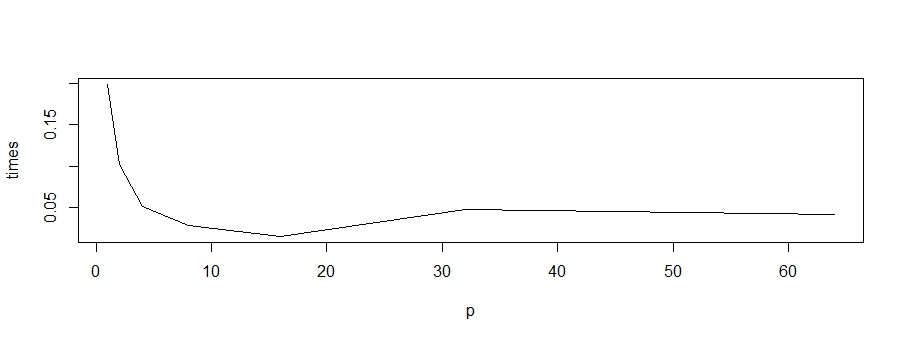
\includegraphics[width=0.6\columnwidth]{Rplot_pi_times_10millions} % Example image
	\caption{Execution time vs number of processors $N = 10^7$ }
\end{figure}

The time decreases inversely to the number of processors. Now lets plot the speedup: 
\begin{figure}[H] % [h] forces the figure to be output where it is defined in the code (it suppresses floating)
	\centering
	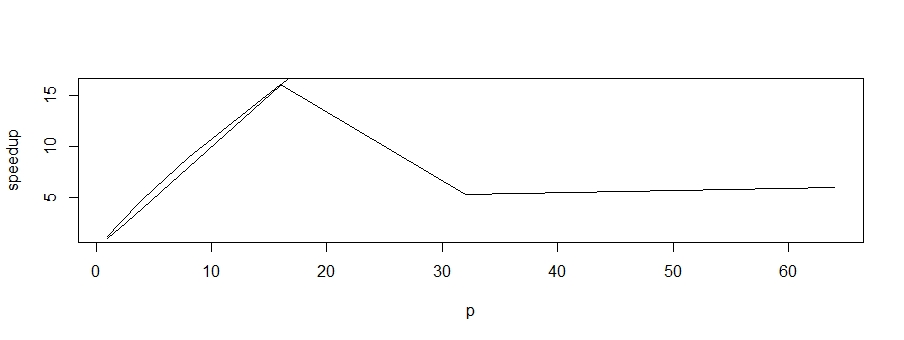
\includegraphics[width=0.6\columnwidth]{Rplot_pi_speedup_10millions} % Example image
	\caption{Speedup vs number of processors $N=10^7$}
\end{figure}
We see that the speedup is not linear: the program runs faster only until around 20 processors.

Let's repeat our observations by having a larger problem size.
Here we have a plot that shows us the maximum \textit{Walltime} processor time against the number of processors. Let us see the case$ N=10^8$:
\begin{figure}[H] 
	\centering
	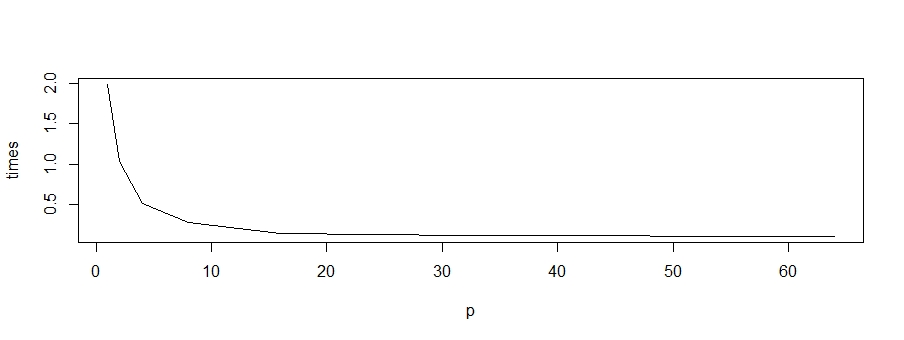
\includegraphics[width=0.6\columnwidth]{Rplot_pi_times_100millions} % Example image
	\caption{Execution time vs number of processors $N= 10^8$}
\end{figure}
\begin{figure}[H] % [h] forces the figure to be output where it is defined in the code (it suppresses floating)
	\centering
	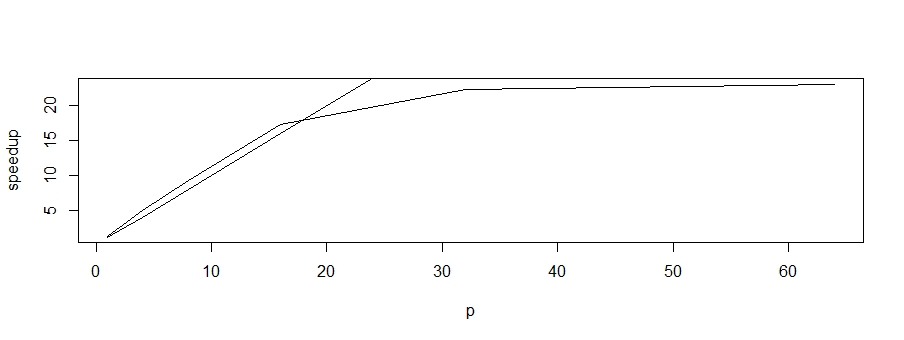
\includegraphics[width=0.6\columnwidth]{Rplot_pi_speedup_100millions} % Example image
	\caption{Speedup vs number of processors $N=10^8$}
\end{figure}
We can observe that the graph is getting closer to the drawn line that represents the perfect speedup (that is speedup = p).
Lets see the same graphs for $N=10^9$:
\begin{figure}[H] % [h] forces the figure to be output where it is defined in the code (it suppresses floating)
	\centering
	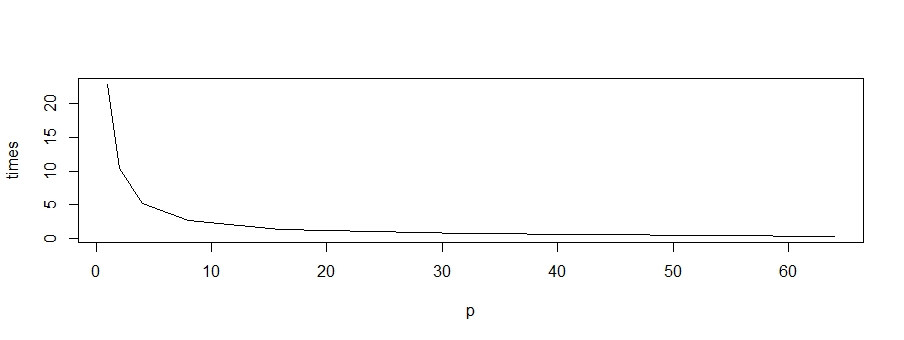
\includegraphics[width=0.6\columnwidth]{Rplot_pi_times_1billion} % Example image
	\caption{ Execution time vs number of processors $N= 10^9$}
\end{figure}
\begin{figure}[H] % [h] forces the figure to be output where it is defined in the code (it suppresses floating)
	\centering
	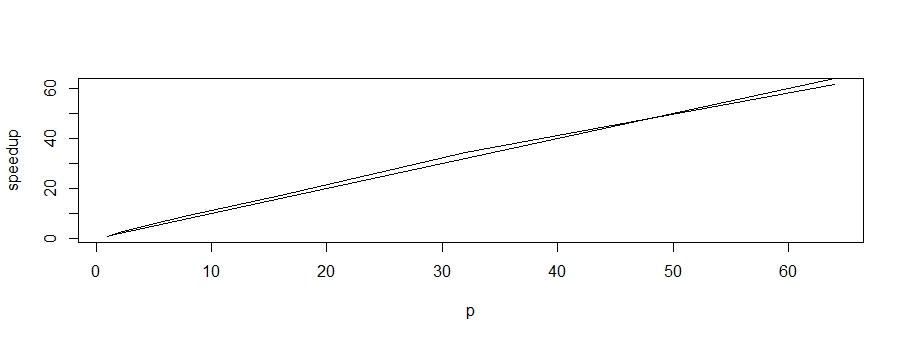
\includegraphics[width=0.6\columnwidth]{Rplot_pi_speedup_1billion} % Example image
	\caption{ Speedup vs number of processors $N= 10^9$}
\end{figure}
Here the speedup plot is linear, for $0 < p < 64$. Adding more processors increases the execution time linearly,at least using the internal time \textit{Walltime}.
\subsection{Using Elapsed Time}
If we use the \textit{Elapsed time} from the command \textit{/usr/bin/time} we get different results:

\begin{figure}[H] % [h] forces the figure to be output where it is defined in the code (it suppresses floating)
	\centering
	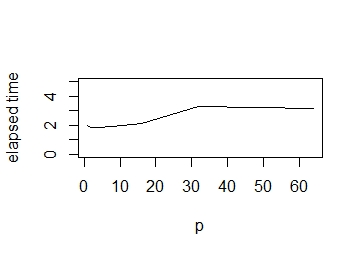
\includegraphics[width=0.6\columnwidth]{Rplot_pi_elapsed_time_10millions} % Example image
	\caption{Elapsed time vs number of processors $N= 10^7$}
\end{figure}
\begin{figure}[H] % [h] forces the figure to be output where it is defined in the code (it suppresses floating)
	\centering
	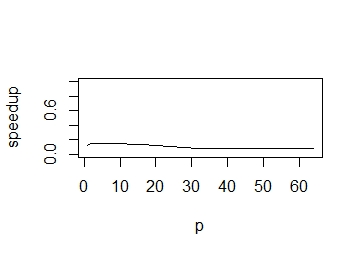
\includegraphics[width=0.6\columnwidth]{Rplot_pi_elapsed_speedup_10millions} % Example image
	\caption{Speedup vs number of processors $N= 10^7$}
\end{figure}

As the problem size increases, we see that the problem scales better, as we see from the following two graphs, calculated with \textit{elapsed\_time} on $N=10^9$:
\begin{figure}[H] % [h] forces the figure to be output where it is defined in the code (it suppresses floating)
	\centering
	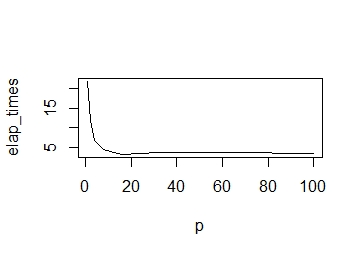
\includegraphics[width=0.6\columnwidth]{Rplot_pi_elapsed_times_1billion} % Example image
	\caption{Elapsed time vs number of processors $N= 10^9$}
\end{figure}
The speedup is calculated by dividing the elapsed time for the serial code by the elapsed times of the parallel code for a different p number of processors. So $speedup = T(1)/T(p)$ as p increases. 
\begin{figure}[H] % [h] forces the figure to be output where it is defined in the code (it suppresses floating)
	\centering
	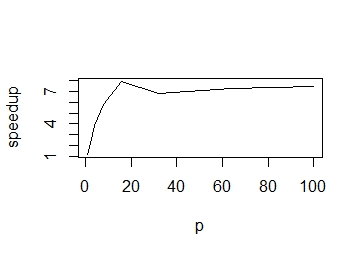
\includegraphics[width=0.6\columnwidth]{Rplot_pi_elapsed_speedup_1billion} % Example image
	\caption{Speedup vs number of processors $N= 10^9$}
\end{figure}

We are considering \textit{Elapsed time} and now the program doesn't scale anymore. This is normal, because the \textit{Elapsed time} reports a more comprehensive time that includes all the overheads that are simply ignored in \textit{Walltime}. The result is thus worse in term of scalability because the parallel time tends to grow as p grows thanks to such overheads. In the end they surpass the time saved by parallelizing the execution.
\subsection{Parallel overhead}

Here we present the model for deducing the overhead of our program. We study the case where $N=10^7$ and we choose to plot the differences between the maximum processor walltime
 and the minimum processor walltime for a growing number of processors.
We obtain the following graph
\begin{figure}[H] % [h] forces the figure to be output where it is defined in the code (it suppresses floating)
	\centering
	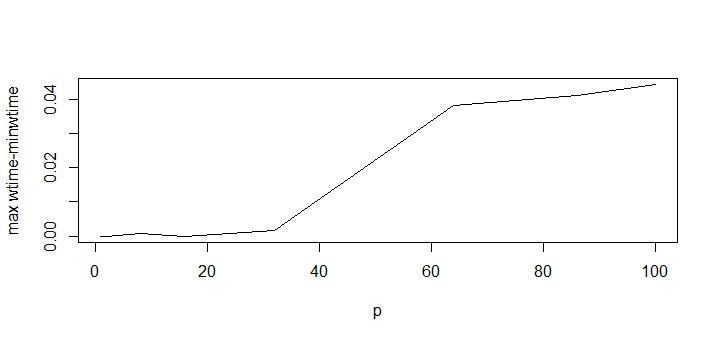
\includegraphics[width=0.6\columnwidth]{Rplot_pi_max_-_min} % Example image
	\caption{Overhead vs number of processors $N= 10^9$}
\end{figure}

We can see that our overhead model grows as p grows. This is explained by the extra computation that is adopted in order to manage more nodes. The growth of the overhead explains why measuring the scalability using \textit{Elapsed time} does not give a scaling result, while the \textit{Walltime} scalability does.
\subsection{Weak scaling}

We run a bash script to automatically collect the execution times for various proportional values of p and N. 
N is equal to $10^7*p$ as p grows.
We obtain the following plot using the maximum\textit{Walltime} time for each number of processors:
\begin{figure}[H] % [h] forces the figure to be output where it is defined in the code (it suppresses floating)
	\centering
	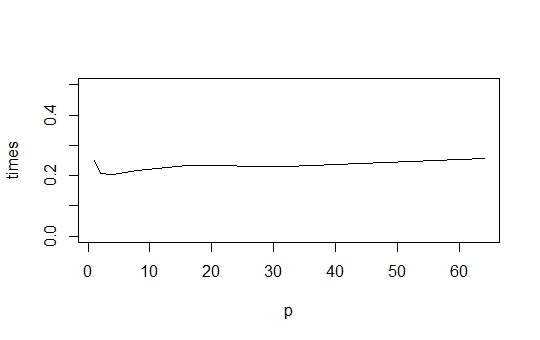
\includegraphics[width=0.6\columnwidth]{Rplot_weak_scaling} % Example image
	\caption{Weak scaling case: execution time vs number of processors $N= 10^7*p$}
\end{figure}
We see that the execution time is almost constant,which is what we expect with a weakly scalable program.The weak scalability aims to enlarge the problem size and the number of processors while leaving the execution time constant.
We get a different result for considering the \textit{Elapsed time} from the \textit{/usr/bin/time} command:
\begin{figure}[H] % [h] forces the figure to be output where it is defined in the code (it suppresses floating)
	\centering
	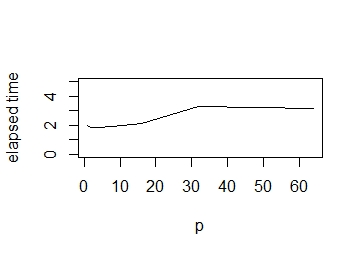
\includegraphics[width=0.6\columnwidth]{Rplot_pi_elapsed_time_10millions} % Example image
	\caption{Weak scaling case: elapsed time vs number of processors $N= 10^7*p$}
\end{figure}
We also plot the speedup we gained by calculating $speedup = T(10^7*p,1)/T(10^7*p,p)$ where $T(N,p)$ is the time calculated on the problem size N and on p processors(the problem size is proportional to the number of processors).
\begin{figure}[H] % [h] forces the figure to be output where it is defined in the code (it suppresses floating)
	\centering
	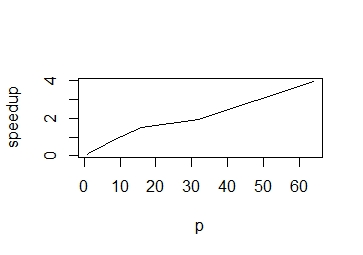
\includegraphics[width=0.6\columnwidth]{Rplot_pi_weak_elapsed_speedup_10million} % Example image
	\caption{Weak scaling case: elapsed time speedup vs number of processors $N= 10^7*p$}
\end{figure}
Here the speedup is somehow linear, showing us that the fact that the elapsed time is almost constant is an advantage in relation to the serial execution time,which instead grows:
\begin{figure}[H] % [h] forces the figure to be output where it is defined in the code (it suppresses floating)
	\centering
	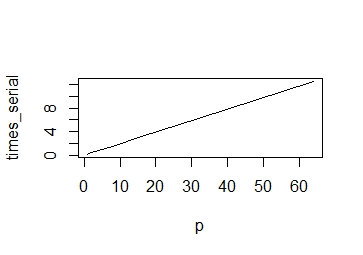
\includegraphics[width=0.6\columnwidth]{Rplot_sum_seq_execution_times} % Example image
	\caption{Serial program case: elapsed time vs number of processors $N= 10^7*p$}
\end{figure}
So the resulting speedup grows because of this distinction between an almost constant elapsed execution time and a linear serial execution time. As the parallel execution time for a growing problem size stays almost the same, the serial code execution time grows,incrementing the speedup and thus making it more convenient to apply the parallelization.
%----------------------------------------------------------------------------------------
\section{Section 3}
Here we have the two c++ codes \textit{sumNumbers\_mpi.cc} and \textit{sumNumbers\_coll.cc}.

The two codes implement the pseudocode we wrote above, including the variations on the assignment . We also don't use any array, but we calculate on the run the addends for the partial sum. Both codes return the sum of N consecutive integers starting from 1 to N and both codes implement the calculation using a parallel approach. Both codes also address the case in which N is not divisible by the number of processors p. In this case the master node takes care of the summation of the integers that are left out from the slave processors. The two codes don't work on one single processor, because the sum needs to be splitted at least among two processors.
The code \textit{sumNumbers\_mpi.cc} uses only \textit{MPI\_Send()} and \textit{MPI\_Recv()}
while the code \textit{sumNumbers\_coll.cc} uses the collective operations \textit{MPI\_Bcast()} and \textit{MPI\_Reduce()} instead. The codes where tested using as an input a file containing the number $N = 10^9$.

We used \textit{MPI\_Walltime()} to collect a few particular subprocess times for $N=10^9$ and $p=10$:

\begin{align} 
	\begin{split}
		&T_{read}= 3.38554 e-05 s\\
		&T_{comp}*(\frac{N}{P})= 0.355836 s\\
		&if N=10^9, P=10\rightarrow T_{comp} = 0.355836/100000000 = 3.5836e-9 s\\
		&T_{comm}=2.14577e-06 s
	\end{split}					
\end{align}
 We see that these values are close to the theoretical values we gave before,making those plausible.
%	EQUATION EXAMPLES
%------------------------------------------------

\section{Section 4}
Now its time to plot the execution time of the function we wrote. We want to test the function's strong scalability.

We consider the \textit{Walltime} execution time for $N=10^9$ and $N=10^{10}$.We start by the \textbf{naive-implemented code}:

\begin{figure}[H] % [h] forces the figure to be output where it is defined in the code (it suppresses floating)
	\centering
	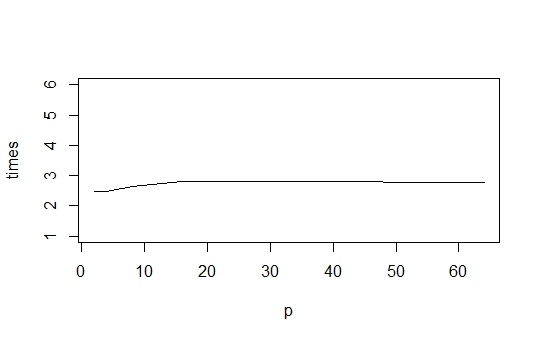
\includegraphics[width=0.6\columnwidth]{Rplot_sum_times_billion} % Example image
	\caption{Walltime execution time vs number of processors $N= 10^9$}
\end{figure}
\begin{figure}[H] % [h] forces the figure to be output where it is defined in the code (it suppresses floating)
	\centering
	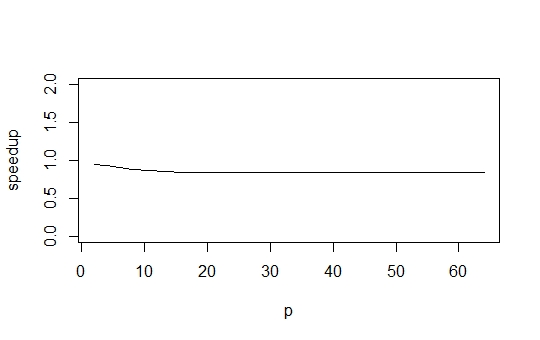
\includegraphics[width=0.6\columnwidth]{Rplot_sum_scalability_billion} % Example image
	\caption{Walltime speedup vs number of processors $N= 10^9$}
\end{figure}

\begin{figure}[H] % [h] forces the figure to be output where it is defined in the code (it suppresses floating)
	\centering
	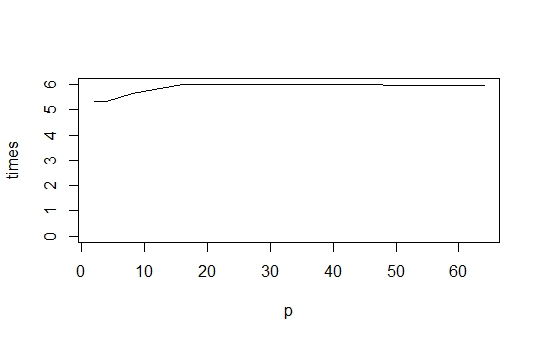
\includegraphics[width=0.6\columnwidth]{Rplot_sum_times_10billion} % Example image
	\caption{walltime execution time vs number of processors $N= 10^{10}$}
\end{figure}
\begin{figure}[H] % [h] forces the figure to be output where it is defined in the code (it suppresses floating)
	\centering
	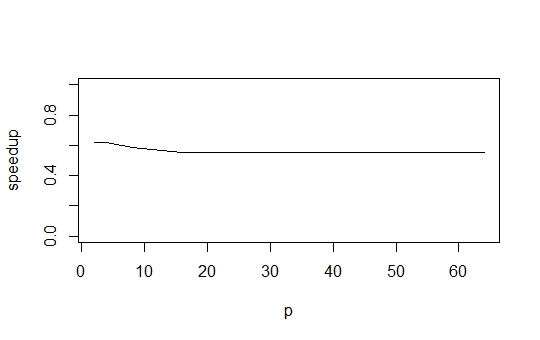
\includegraphics[width=0.6\columnwidth]{Rplot_sum_speedup_10billion} % Example image
	\caption{walltime speedup vs number of processors $N= 10^{10}$}
\end{figure}

We see that the program isn't scaling as we predicted in our model.
Where by $10^10$ the theoretical model was scaling perfectly, our model is instead not scaling.
The execution time seems to be constant.
The executed program was the naive-implemented one,and probably the communication time increases too much and nullifies the time saved throughout the parallelization. 

We should also consider that the partial sums consists of more than one single floating point operation. So our program places more time on the computation part of the execution than our model. A better model would reconsider the formula for the parallel execution time $T_p$. Like for example $T_p = T_{read} + (p-1+n_{sum}*n/p+n_{serial})*T_{comp}+2*T_{comm}(p-1)$ where $n_{sum}$ represents the number of floating point operations required to calculate a single addend and $n_{serial}$ represent the floating point operations that are used to calculate the variable \textit{subarray\_size},which is the size of the subproblem.This could be an example on how to make a best theoretical model that, by having a larger $T_p$, will avoid scaling for a larger problem size N. 


But here basically adding more processors does not speed up the execution time, and the program is poor at parallelizing the task at hand. Let's also see the case of \textit{Elapsed time},from which we draw the same conclusions:

\begin{figure}[H] % [h] forces the figure to be output where it is defined in the code (it suppresses floating)
	\centering
	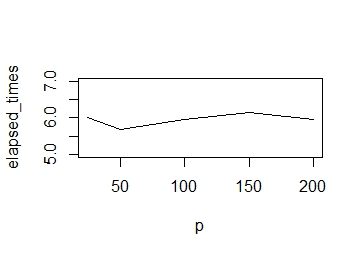
\includegraphics[width=0.6\columnwidth]{Rplot_sum_elapsed_time} % Example image
	\caption{Elapsed time execution time vs number of processors $N= 10^9$}
\end{figure}

\begin{figure}[H] % [h] forces the figure to be output where it is defined in the code (it suppresses floating)
	\centering
	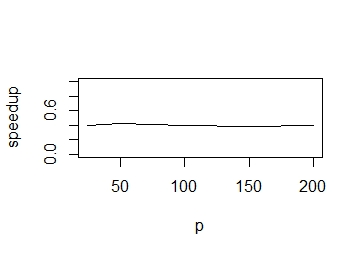
\includegraphics[width=0.6\columnwidth]{Rplot_sum_elapsed_speedup} % Example image
	\caption{Speedup of the elapsed time vs number of processors $N= 10^9$}
\end{figure}
%----------------------------------------
%\begin{figure}[H] % [h] forces the figure to be output where it is defined in the code (it suppresses floating)
	%\centering
	%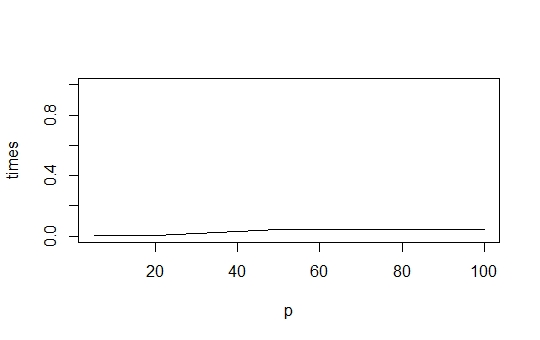
\includegraphics[width=0.6\columnwidth]{Rplot_sum_times_thousand} % Example image
	%\caption{execution time vs number of processors $N= 10^3$}
%\end{figure}
We get a better result if we plot the scalability for the \textbf{sumNumbers\_coll.cc} code, with $N=10^{9}$. The time taken is the \textit{Walltime} given by \textit{MPI\_Walltime()}:

\begin{figure}[H] % [h] forces the figure to be output where it is defined in the code (it suppresses floating)
	\centering
	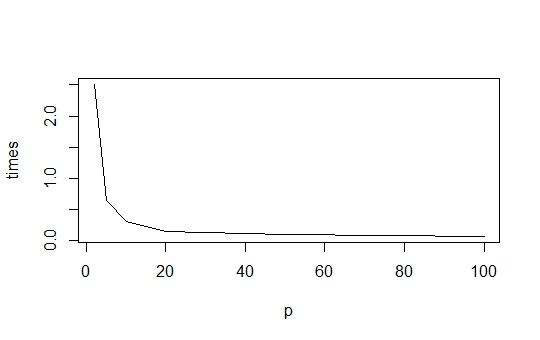
\includegraphics[width=0.6\columnwidth]{Rplot_complex_sum_times_1billion} % Example image
	\caption{Walltime execution time vs number of processors $N= 10^9$}
\end{figure}

\begin{figure}[H] % [h] forces the figure to be output where it is defined in the code (it suppresses floating)
	\centering
	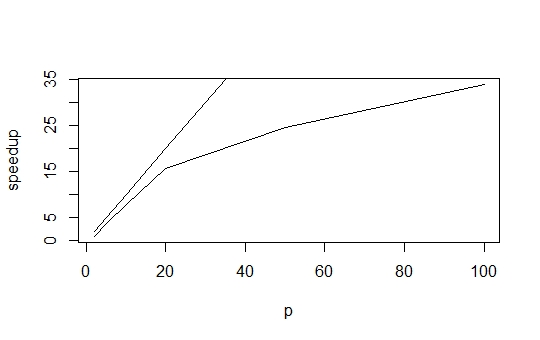
\includegraphics[width=0.6\columnwidth]{Rplot_complex_sum_speedup_1billion} % Example image
	\caption{Walltime speedup vs number of processors $N= 10^9$}
\end{figure}
We see that this second code scales better than the first one.
We replicated the results with $N=10^{12}$,although there is no common data type to store the result of the sum and although we couldn't test a simple serial code of the summation with such a big number. We estimate that for $N=10^{12}$ then $T(1) = 5 s$.
\begin{figure}[H] % [h] forces the figure to be output where it is defined in the code (it suppresses floating)
	\centering
	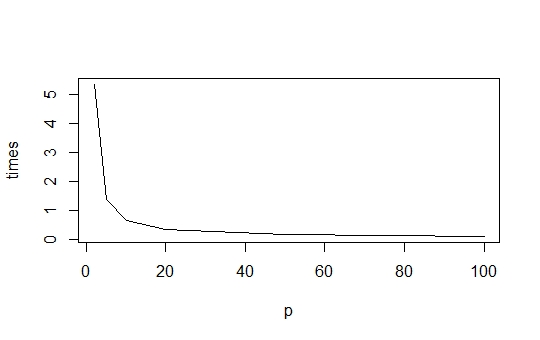
\includegraphics[width=0.6\columnwidth]{Rplot_complex_sum_times_trillion} % Example image
	\caption{Walltime execution time vs number of processors $N= 10^{12}$}
\end{figure}
\begin{figure}[H] % [h] forces the figure to be output where it is defined in the code (it suppresses floating)
	\centering
	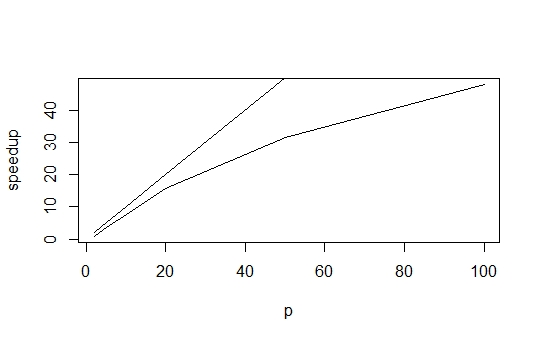
\includegraphics[width=0.6\columnwidth]{Rplot_complex_sum_speedup_trillion} % Example image
	\caption{Walltime speedup vs number of processors $N= 10^{12}$}
\end{figure}
We can deduce that the code is somehow scaling as N grows.Maybe if N is large enough we would see that the program scales.
\subsection{\textbf{Elapsed time} case}
Let's also plot the \textbf{Elapsed time} of the \textbf{sumNumbers\_coll.cc} code for $N=10^7$ to make a comparison:

\begin{figure}[H] % [h] forces the figure to be output where it is defined in the code (it suppresses floating)
	\centering
	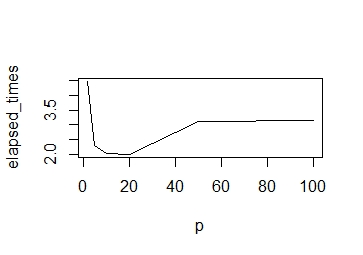
\includegraphics[width=0.6\columnwidth]{Rplot_sum_elapsed_times_10millions} % Example image
	\caption{Elapsed time vs number of processors $N= 10^7$}
\end{figure}
\begin{figure}[H] % [h] forces the figure to be output where it is defined in the code (it suppresses floating)
	\centering
	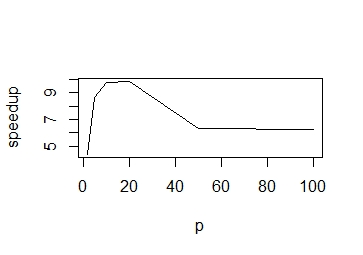
\includegraphics[width=0.6\columnwidth]{Rplot_sum_elapsed_speedup_10millions} % Example image
	\caption{Speedup of the elapsed time vs number of processors $N= 10^7$}
\end{figure}
We see that the code doesn't scale for this problem size either.
Since \textbf{Elapsed time} adresses a wider execution time, we expected a worse result. We can also see the case $N=10^9$:
\begin{figure}[H] % [h] forces the figure to be output where it is defined in the code (it suppresses floating)
	\centering
	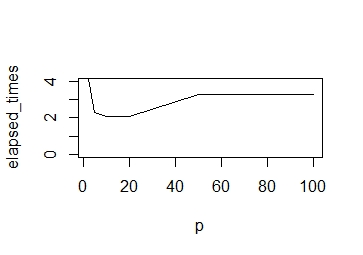
\includegraphics[width=0.6\columnwidth]{Rplot_sum_elapsed_times_1billion} % Example image
	\caption{Elapsed time vs number of processors $N= 10^9$}
\end{figure}
\begin{figure}[H] % [h] forces the figure to be output where it is defined in the code (it suppresses floating)
	\centering
	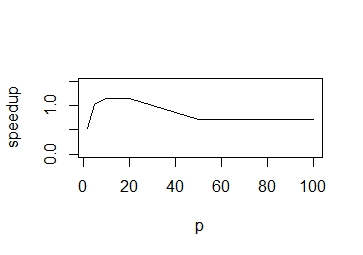
\includegraphics[width=0.6\columnwidth]{Rplot_sum_elapsed_speedup_1billion} % Example image
	\caption{Speedup of the elapsed time vs number of processors $N= 10^9$}
\end{figure}

We are increasing the size of the problem, yet the code doesn't scale. We conclude that there must be a problem in the initialization of the code. The parallelization is not effective in reducing the execution time . Adding more processors does not speed up the execution time.
This is because the \textit{elapsed time} counts the overhead time too, while just using \textit{walltime} returns us the execution time of the portion of the code that scales better. In the end they are different measurements that take into account different parts of the execution, and yet the elapsed time is the best one because it returns a time that measures even the overhead,which is fundamental in assessing the program's scalability, and thus its performance as a parallel problem.
%------------------------------------------------
We must conclude that the code we wrote is not good at parallelizing the problem, although we focused on making it as close as possible to the assignment's description. The code itself works well in calculating the sum of N integers from 1 to N,but yet the code does not parallelize well. We see that there is a difference between a good-working code and an efficient one. 


%----------------------------------------------------------------------------------------
%	LIST EXAMPLES
%------------------------------------------------------------------------------


%----------------------------------------------------------------------------------------

%-------------------------------------------------------------

%------------------------------------------------

%----------------------------------------------------------------------------------------

\end{document}
